% Font size, paper type
\documentclass[12pt]{article}
% Aesthetic margins
\usepackage[margin=1in]{geometry}
% Core math packages,
% Mathtools loads amsmath, and amsmath gives basic math symbs
% Amsfonts & amssymb are misc. symbols you might need
\usepackage{mathtools, amsfonts, amssymb}
% Links in a pdf
\usepackage{hyperref}
% Use in pictures, graphs, and figures
\usepackage{graphicx}
% Header package
\usepackage{fancyhdr}
% Underlining with line breaks
\usepackage{ulem}
% Adjust accordingly given warning messages
\setlength{\headheight}{15pt}
% So we can more easily format text with pictures
\usepackage{float}

% Sets footer
\pagestyle{fancy}
% Removes default footer style
\fancyhf{}

\rhead{
  Shengdong Li
  Calc 3
}

\rfoot{
  Page \thepage
}

% Makes links look more appealling
\hypersetup{
    colorlinks=true,
    linkcolor=blue,
    filecolor=magenta,      
    urlcolor=cyan,
}

% \usepackage{indentfirst}

\begin{document}
\title{Response to Adithi Mahankali}
\author{by Shengdong Li}
\date{17 December 2020}
\maketitle

Hey Adithi,
Thank you so much for responding to my initial post!

Your comments about the properties of the Epicycloid curve compared to the asteroid curve were very insightful and gave me a lot of clues as to why I observed the graph changing in regard with respect to the constants.
\begin{quote}
  ``I believe the entire graph stretches and shrinks rather than just a horizontal or vertical change because the constant is being multiplied by both the $x$ parameter and the $y$ parameter''
\end{quote}
I definitely agree with your point here on my graph, in both
\begin{align*}
  x\left(t\right)&=\left(a+b\right)\cos t-b\cos\left(\left(\frac{a}{b}+1\right)t\right)\\
  \intertext{\centering and}
  y\left(t\right)&=\left(a+b\right)\sin t-b\sin\left(\left(\frac{a}{b}+1\right)t\right)
\end{align*}
the $\left(a+b\right)$ was attached to $\cos(t)$ and $\sin(t)$ respectively, along with $b$ attached to the second term of each as well. Therefore, the entire graph would definitely be increased in size based off of $a$ and $b$.
\begin{quote}
  ``I also think that when the constants are inside the function such as sin(at), which is how your curve was, the number of petals or points change as well.''
\end{quote}
I think that your point about constants being inside of the sinusoids is really interesting, especially since your astroid curve did not have constants inside the sinusoids, and had fixed points. 

This also makes sense because the parametric equation for a circle also has $r\sin t$ and $r\cos t$, but because there is no constant inside, increasing $r$ just changes the size of the circle. I tried adding a single $a$ value to the inside of the $\cos(t)$ in the $x(t)$ of a circle to make
$$
c\left(t\right)=\left(\cos\left(at\right),\sin\left(t\right)\right)
$$
\begin{center}
then set 
\end{center}
$$
a=1.1
$$
and that turned it from a circle with one curve to a square-like shape with a ton of curves.
\begin{figure}[H]
  \begin{center}
    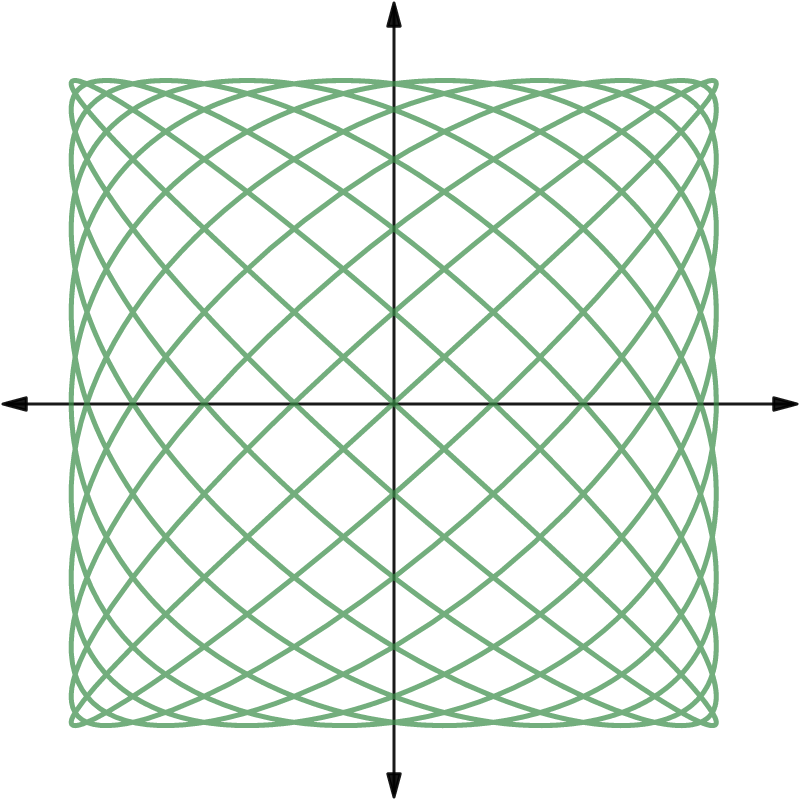
\includegraphics[scale=.3]{square.png}
    \caption{\textit{Graph of $c\left(t\right)=\left(\cos\left(at\right),\sin\left(t\right)\right)$.} Desmos link \href{https://www.desmos.com/calculator/z4lbq0xn0a}{\textcolor{blue}{here}}}
  \end{center}
\end{figure}

Thanks for replying again,
I'll make sure to take a closer look at the asteroid graph as well!
\bigskip

Cheers,

- Andy
\end{document}